\documentclass[../main.tex]{subfiles}
\graphicspath{{\subfix{../}}}
\begin{document}

\chapter{How to Create an IMF Model}
\label{ch:How to Create an IMF Model}
This chapter gives an introduction and
step by step guideline of how to create an IMF model. Prior understanding of IMF as a framework and language is
assumed. Acquaintance with IEC/ISO~81346 is beneficial, but not required. When explaining modelling and advising on
different approaches, some examples are provided to make the explanations more concrete. These examples cover only a
few of the possible use cases; the application of IMF modelling spans a much larger range.

\section{What it Means to Create an IMF Model}

To create an IMF model of the simple fluid separation system shown in \autoref{fig:Figure 30}, means
to specify the functional requirements, the spatial arrangement, and the
specification of a realisation of this system. This is done not by diagrams or drawing documents, but by
creating an information model: by composing a structure of building blocks with relations, both in hierarchy
(vertical) and in topology (horizontal), and assigning attributes with values. The level of detail that is put into it---the granularity of the model---is dependent
on the use case. This applies both to the detail of structure that is composed, as well as the extent to which
attributes are assigned.

\begin{figure}[htb]
  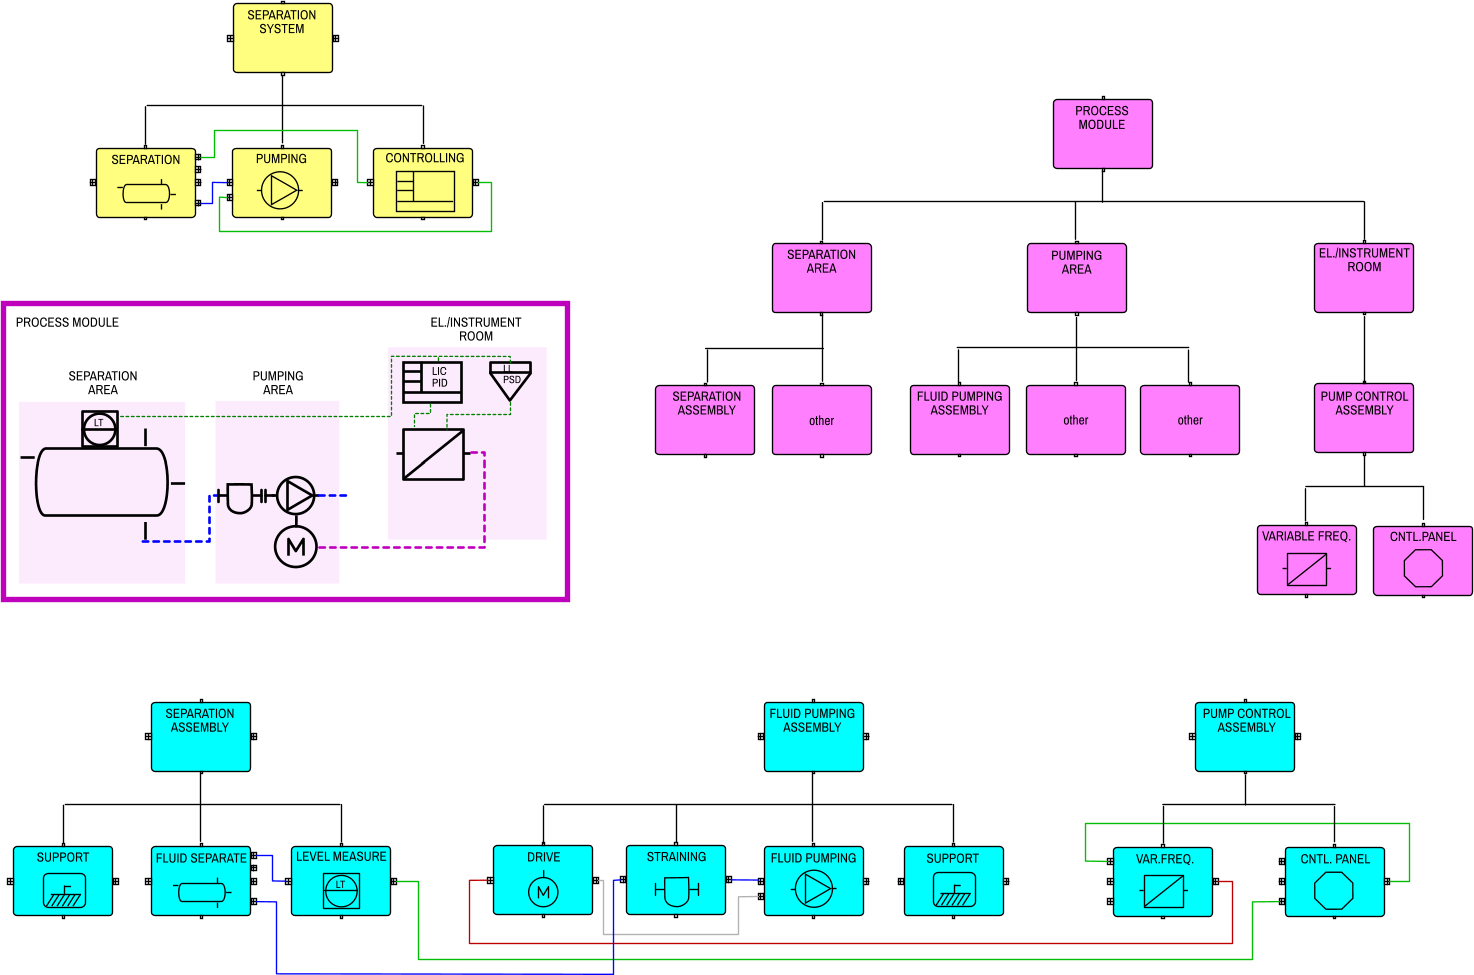
\includegraphics[width=1\textwidth]{img/IMFmanual-img049.png}
  \caption[A separation system represented as an IMF model.]{A separation system represented as an IMF model with
    three aspects: Function, Location, and Product.}
  \label{fig:Figure 30}
\end{figure}

When creating an IMF model as part of establishing an early phase concept, the modelling can be at a very high level of abstraction
and maybe only include the functional requirements. On the other hand, when creating an IMF model of a specific
solution, such as a manufacturer's documentation of a pumping solution, the model can be very detailed and include
all features of the pumping assembly. It is essential to understand the purpose of the modelling in each individual
use case and how this gives guidance to the best modelling approach.

\subsection{Incorporating Modelling into an Established
  Work Process}
Established work processes for engineering and design are often directed towards creating
diagrams, drawings, and texts contained in documents which have a defined and fixed information scope. Typically,
such a document only addresses one discipline, i.e., only process or only electro, and often only one sub-section of
the facility asset. The level of detail is generally dictated by the type of document, e.g., an overall single line
diagram will only contain information about the main pathways of the electrical distribution system.

The fixed information scope of established document types, contrasts with the flexible information scope of an IMF
model. During the transition of work processes from a document-based to a model-based way of working there is a need to
bridge between the two paradigms by referring to legacy document types when scoping a modelling exercise. For
example, the scope for modelling is to define the same level of information content for the facility asset as
typically represented in a process flow diagram (a document type). As the industry gains experience from the
transition from document-based to model-based, new work processes can be developed that are directed towards
continuously enriching an information model rather than producing fixed format information.

When modelling a facility asset there are three different roles or mind-sets to choose from, depending on use case and
life cycle phase:

\begin{enumerate}
  \item Defining needs: setting requirements.
  \item Specifying solution: fulfilling requirements.
  \item Documenting the actual installation (or assembly, equipment, device, component).
\end{enumerate}
The dividing line between requirements and specification is not always distinct, but in this context, requirements are
about what is needed, whereas specification is about how to achieve it. In some use cases, such as when
re-documenting an existing facility asset, the setting of requirements and specifications may have to be reverse
engineered, based on the as-built documentation.

\subsection{Defining a Need: Setting requirements}
When developing a new facility asset, the first thing that must be done is to define the
functional requirements, i.e., `what is needed'. Essentially this is about what \emph{activity} is needed, broken
down into the individual activities it comprises. Taking the above separation plant given in \autoref{fig:Figure 30} as an example,
the main activity needed of the facility asset is Separation, and the sub-activities are 3-Phase Separation,
Pumping, and Controlling. Each of these activity needs are further characterised by means of their attributes,
e.g., the pumping attribute Volumetric Flowrate = 200 m\textsuperscript{3}/h.

Activity requirements are captured in the Function Aspect whereas requirements that are given by the intended location
are captured in the Location Aspect.

\subsection{Specifying a Solution: Fulfilling Requirements}
When specifying solutions that fulfil the requirements, the objective is to describe how
to achieve the activities required, by means of components, equipment, and assemblies. The specified solutions must
not only fulfil the activity requirements, but also the requirements given by the intended location, as well as any
overall requirements that apply. Referring to the separation plant given in \autoref{fig:Figure 30}, the required pumping of 200
m\textsuperscript{3}/h must be fulfilled, say by a centrifugal pump with a capacity of 300 m\textsuperscript{3}/h,
which is suitable for location in the pumping area by being waterproof, and by meeting the standard API 611
(background) requirements.

Solution specifications are captured in the Product Aspect whereas specifications of the space of the solutions and
their positions are captured in the Location Aspect.

\subsection{Documenting the Actual Installation}
Setting requirements and specifying solutions describes the intended facility asset. Once
the specified components, equipment, and assemblies have been manufactured, delivered, or installed they can be
documented by enriching the IMF model with the actual information about the physical objects themselves. Thus, it can
be documented that the specifications are met. The typical example is that the above centrifugal pump may have a
nameplate capacity of 350 m\textsuperscript{3}/h and a serial number 5270-2565.

Documentation of actual physical objects and their installation is captured in the Installed Aspect.

\section{Before one Starts to Model}
Before starting to model, we need to be clear on the purpose or \emph{interest} of the
modelling. The interest should be defined based on the end user needs, or the user needs next in the value chain.
Often this is given by the work process the user is executing at this point in the lifecycle. \autoref{fig:Figure 31} illustrates
a separation system, shown as a conceptual diagram and as an imagined real solution.

\begin{figure}[htb]
  \centering
  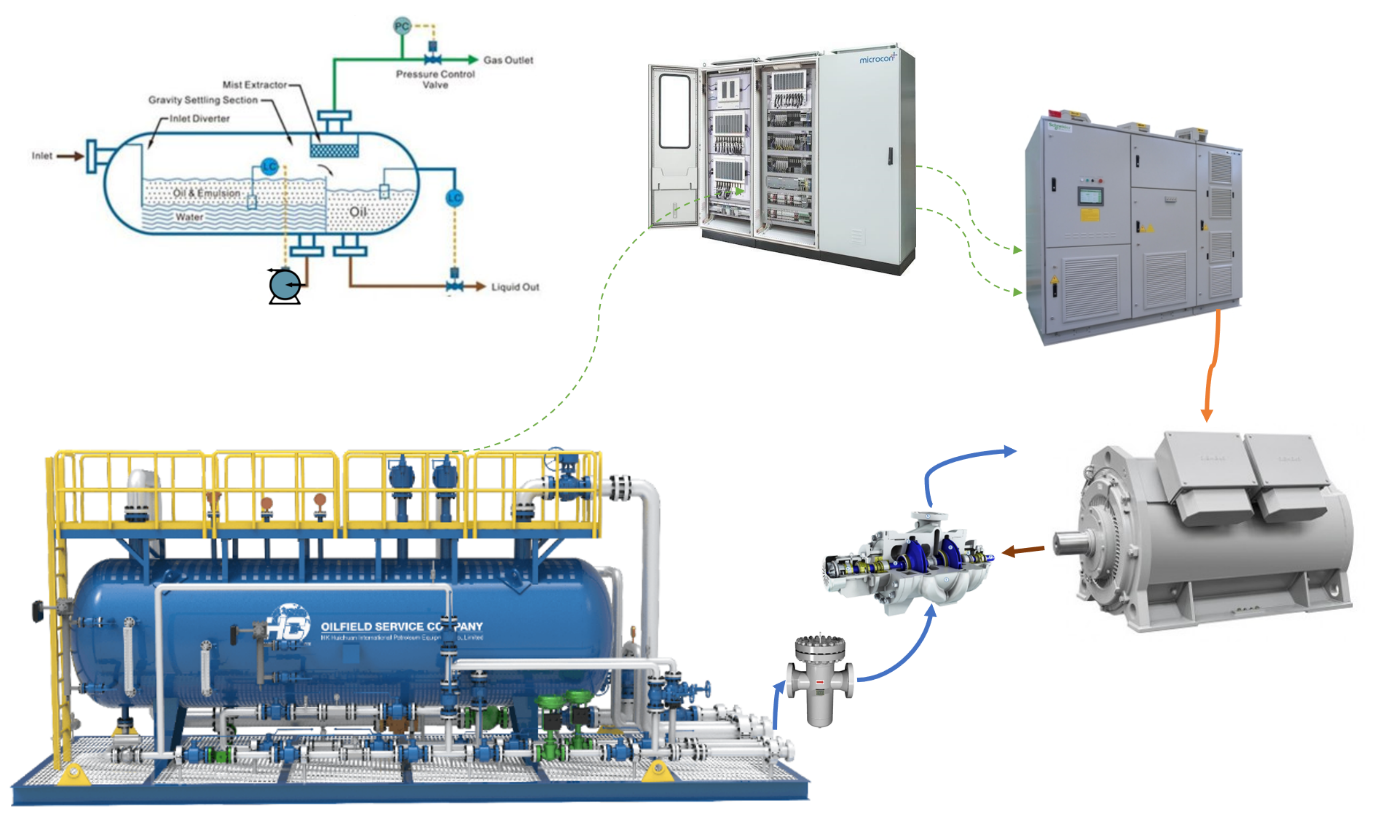
\includegraphics[width=1\textwidth]{img/IMFmanual-img050.png}
  \caption{A separation system shown as a conceptual diagram and as an imagined real solution.}
  \label{fig:Figure 31}
\end{figure}

\subsection{Defining the Interest of the Model}
The interest of the modelling can range from defining requirements at a conceptual level to documenting the actual facility asset as installed. Likewise, the interest can be to model the automation and
control part of the solution, or the fluid processes. In other cases, the interest is to model a multi-discipline
multi-aspect model at a high level of aggregation to provide a skeleton for later more detailed modelling.

Always begin by understanding and stating the interest of why and what to model.

\subsection{Framing the Overall Requirements}
As for any engineering and design effort there are overall requirements that must be
identified and evaluated to understand how they apply. The volume of such requirements increases with the level of
detail of the modelling, but even for high level functional requirements modelling they must be considered. As an
example, this could be safety requirements for systems and solutions that handle high pressure hydrocarbon fluids. `Overall requirements' means any information that has this purpose, in general they are found outside of the model, in documents, authority requirements, etc. To include these into the IMF model may only be feasible by using, say an IMF type Requirements Link which contains a link to the external documentation of the requirements, but in the future such requirements could be implemented as a model.

\subsection{Framing the Prior Governing Requirements}
Usually, at an earlier stage, specific requirements and possibly also solution
specifications have been developed, either captured in documents or as a facility asset model. This information must
be understood as it governs the modelling when it continues.

\subsection{Outlining the Scope of the Model and its Outside Interfaces}
IMF has a default taxonomy for granularity levels which can be employed to define the
intended level of detail. This taxonomy is defined by ISO/IEC~81346-O\&G~\cite{81346-OG} which specifies the three levels:

\begin{enumerate}
  \item Field wide (represented by a single letter code).
  \item Technical system (represented by a two-letter code).
  \item Component (represented by a three-letter code).
\end{enumerate}
There may be a need for additional and more fine-grained taxonomies, such as that specified by ISO~14224~\cite{14224} or other
industry standards or conventions. Granulation detail levels are not the same as system breakdown levels. For
example, in an information model of a facility asset, a technical system can be part of another technical system.
With IMF being an open format, it is up to the user to employ the most fit-for-purpose taxonomy (that can consist of
one or several) to define the intended scope and detail of the modelling.

Likewise when defining the scope, it is important to define the outer interfaces, that is, stating where does this model end
(and where another model continues?) Such interfaces include upstream and downstream interfaces as well as interfaces
between different disciplines, between aspects, or between IMF models.
It is possible, but not recommended, to begin modelling without having decided how deep in granularity to go, or how wide in scope to span, but this would not be best practice (indeed it is not best practice for any kind of effort). Good planning of the work would include to target a specific scope and a specific level of detail.

\section{How to Choose which Aspect to Begin with}
A proposed sequence of aspects is:

\begin{center}
  Function $\Rightarrow$ Product $\Rightarrow$ Location $\Rightarrow$ Installed
\end{center}

However, it is often both necessary and valuable to iterate between aspects, or between setting required activities,
specifying fulfilling solutions, and defining and allocating space and locations. It may help structure the work
process to choose which aspect to begin with and think of as the `master' aspect.

\begin{figure}[htb]
  \centering
  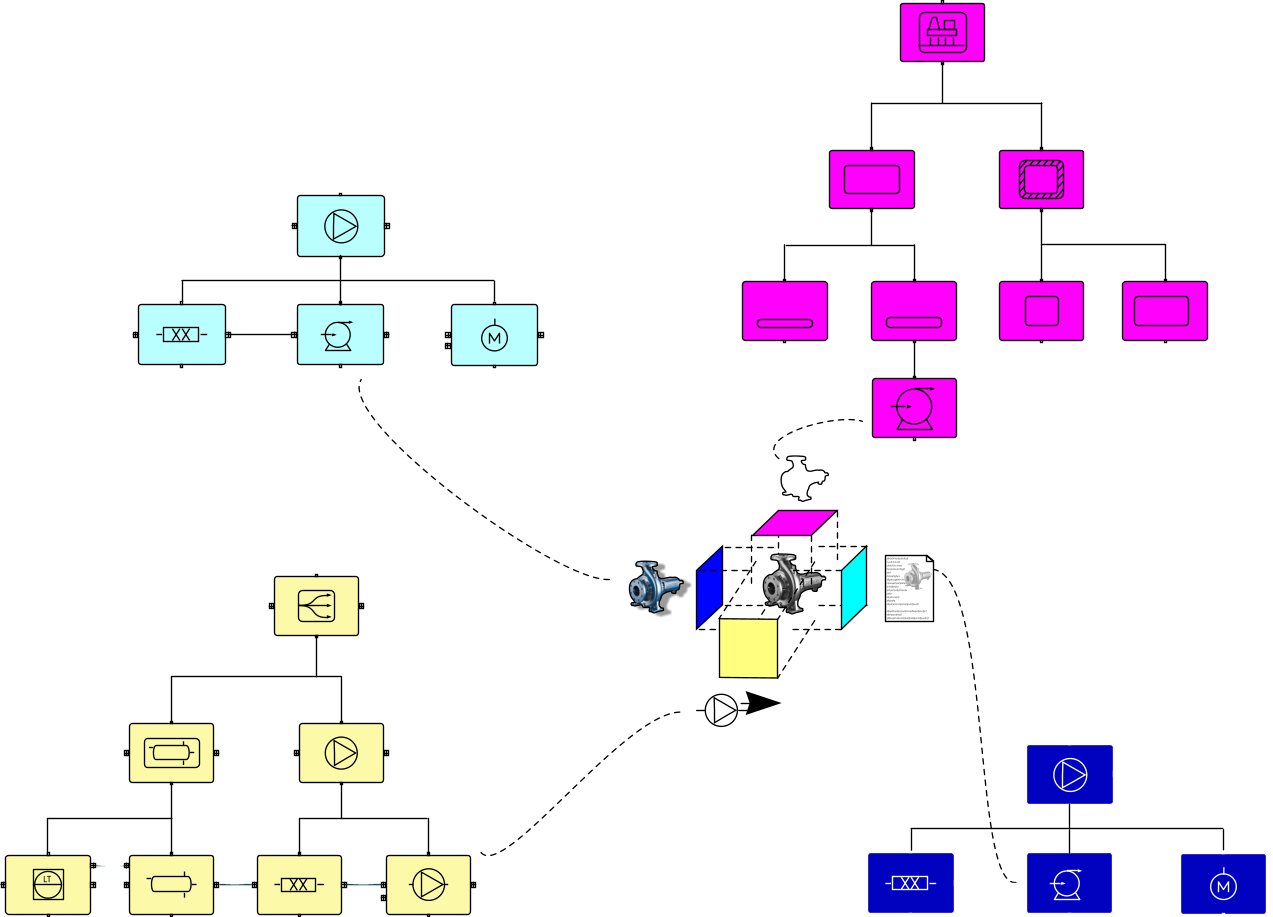
\includegraphics[width=.9\textwidth]{img/IMFmanual-img051.png}
  \caption[A pump system represented as an IMF model using four aspects.]{A pump system represented as an IMF model using four aspects: Function, Location, Product, and Installed.}
  \label{fig:Figure 32}
\end{figure}

\subsection{The Function Aspect}
Choose the Function Aspect when the objective is to set requirements to activities (what
it is going to perform) of the facility asset. Often this is logically the first step.

Move from the Function Aspect when required activities have been defined to a level of detail that solutions can
be specified to fulfil them.

\subsection{The Product Aspect}
Choose the Product Aspect when the objective is to specify solutions comprising
components, equipment, or assemblies. Often is this the logical second step, assuming the first step has been to set
requirements. When creating a model of an already existing design this is the first step. To specify a solution may
take place in several steps: first by the engineering contractor as part of a procurement process, secondly by the
vendor or manufacturer as part of a bidding process, and sometimes also in further steps involving special expertise
on topics such as materials technology.

Move from this aspect at the latest when the solution has been sufficiently specified for procuring/acquiring.

\subsection{The Location Aspect}
The Location Aspect can represent the physical architectural/construction
perspective, meaning modules, rooms, decks, areas, etc., with their X, Y, Z coordinates and characteristics. When
modelling, choose the Location Aspect when the objective is one of two:

\begin{enumerate}
  \item to specify the spatial and positional properties of a component, equipment, or assembly.
  \item to state the requirements that apply within the given location: area restrictions, e.g., noise limitations,
        ambient conditions, etc.
\end{enumerate}
Modelling in this aspect depends on knowledge about what will eventually be needed to be located, both the size,
weight and suitability for ambient conditions, as well as safety, access, and maintenance needs. Therefore, the
modelling in this aspect depends on the use case and work processes.

Move from the Location Aspect when locations and their requirements have been defined to a level of detail that
solutions can be specified to meet them.

\subsection{The Installed Aspect}
When modelling, choose the Installed Aspect when the objective is to document the physical
reality, i.e., the actual component, equipment, or assembly. Contrary to what the name of this aspect indicates it
does not have to be actually installed (on site) in order to be documented thus. It must have been manufactured/made.
In other words, it must exist. This means that this aspect can also be used to document components, equipment,
or assemblies that are in storage, possibly as spare parts.

This aspect is different from the three aspects above in that it does not \emph{model} the facility asset, it
\emph{documents} it.

\section{How to Decide which Modelling
  Approach to use}
\label{ch:Chapter 5.4}
There are different approaches for how to model, with regards to where to begin and in
which direction to progress. In the following sections we will use the IMF model given in \autoref{fig:Figure 33} to illustrate the
different approaches.

\begin{figure}[htb]
  \centering
  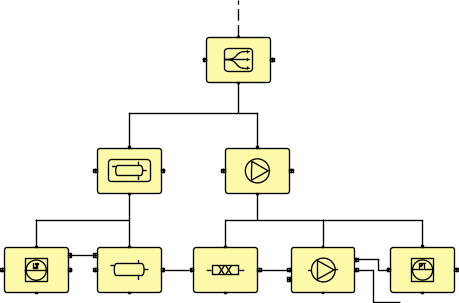
\includegraphics[width=.5\textwidth]{img/IMFmanual-img052.png}
  \caption{An example of an IMF model.}
  \label{fig:Figure 33}
\end{figure}

The approach to select for a given case is to some extent use case driven, but there are multiple case-to-case
conditions that influence the optimal approach. Unless there are clear arguments for doing otherwise, the default
choice should be the top-down approach.

\subsection{A Top-down Modelling Approach}
\begin{figure}[htb]
  \centering
  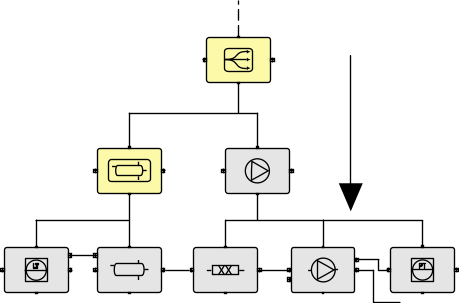
\includegraphics[width=.5\textwidth]{img/IMFmanual-img053.png}
  \caption[A top-down modelling approach.]{A Top-down modelling approach. (Grey
colouring indicates blocks yet to be modelled.)}
  \label{fig:Figure 34}
\end{figure}

The top-down approach shown in \autoref{fig:Figure 34}, closely mirrors the systems engineering methodology, i.e., breaking higher
level systems down into their constituent sub-systems, iteratively refining and detailing the model. It allows
someone with a high-level understanding of the facility asset requirements to establish a design basis which
thereafter can be further detailed by someone with more specialised expertise on individual sub-systems. 

\subsection{A Bottom-up Modelling Approach}
\begin{figure}[htb]
  \centering
  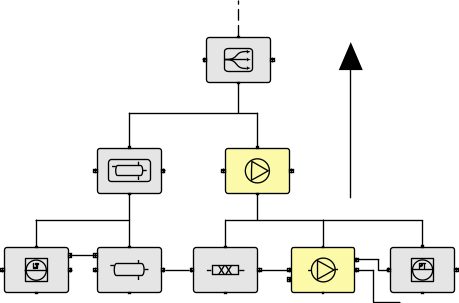
\includegraphics[width=.5\textwidth]{img/IMFmanual-img054.png}
  \caption[A bottom-up modelling approach.]{A bottom-up modelling approach. (Grey colouring indicates blocks yet to be modelled.)}
  \label{fig:Figure 35}
\end{figure}

The bottom-up approach shown in \autoref{fig:Figure 35}, supports the process of integrating sub-systems into higher-level systems
in an optimal way. Typically, this is needed if any sub-systems are predefined in some way, usually because they
represent standardised or off-the-shelf systems. 

\subsection{A Follow-Stream Modelling Approach}

\begin{figure}[htb]
  \centering
  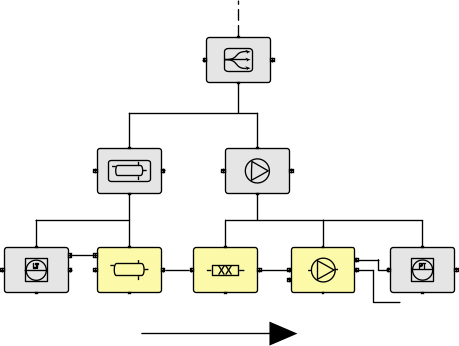
\includegraphics[width=.5\textwidth]{img/IMFmanual-img055.png}
  \caption[A follow-stream modelling approach.]{A follow-stream modelling approach. (Grey colouring indicates blocks yet to be modelled.)}
  \label{fig:Figure 36}
\end{figure}

The follow-stream approach shown in \autoref{fig:Figure 36}, allows full attention to how media shall stream into and through the
facility asset, ultimately resulting in the required media output. Following this approach, the view taken is that
the individual sub-systems are only a means for defining input(s) and output(s) and the required transformation in
between. What results from this approach is therefore a topology (horizontal connections). To finish such a model
will require a bottom-up integration modelling effort. 

\subsection{A Follow-thread Modelling Approach}
\begin{figure}[htb]
  \centering
  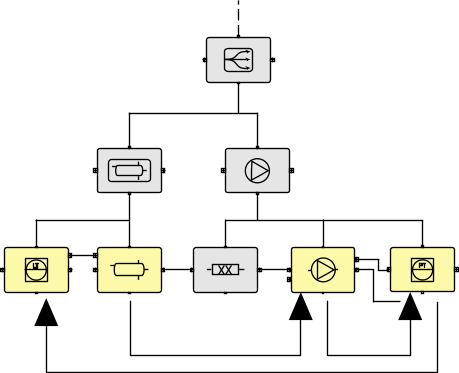
\includegraphics[width=.5\textwidth]{img/IMFmanual-img056.png}
  \caption[A follow-thread modelling approach.]{A follow-thread modelling approach. (Grey colouring indicates systems that do not have primary focus or that do not
yet exist.)}
  \label{fig:Figure 37}
\end{figure}

Illustrated in \autoref{fig:Figure 37}, the follow-thread approach is well suited for multidisciplinary modelling. The threads can be
explained as:

\begin{enumerate}
  \item Separation is required, and for it to work optimally a pump is needed.
  \item For the pump to do its duty it needs a control system.
  \item For the control system to work it needs a level sensor which is connected to the separator.
\end{enumerate}
The disciplines involved in this thread are process, process control, and instrumentation. What results from this
approach is therefore a thread of defined dependencies between systems, and to finish such a model will require a
bottom-up integration modelling effort. 

\section{How to Create and Connect Aspect Elements}
The building blocks of an IMF model are the various types of aspect elements: blocks and terminals with aspects. The aspect elements are fetched from a library, or more precisely they are created or instantiated from IMF types that reside
in a IMF type library. When an aspect element is instantiated from an IMF type, it has several attributes already defined,
reflecting what it represents. For example, an aspect element Pumping should, e.g., have an attribute
named Volumetric Flowrate and other attributes that characterises the pumping activity.

To compose a model requires creating aspect elements and connecting them. This is done by placing them into
a breakdown hierarchy and topology, and by defining relations to aspect elements
in other aspects. Depending on the modelling approach chosen, all of these different types of connections may not
need to be defined initially.

\begin{figure}[htb]
  \centering
  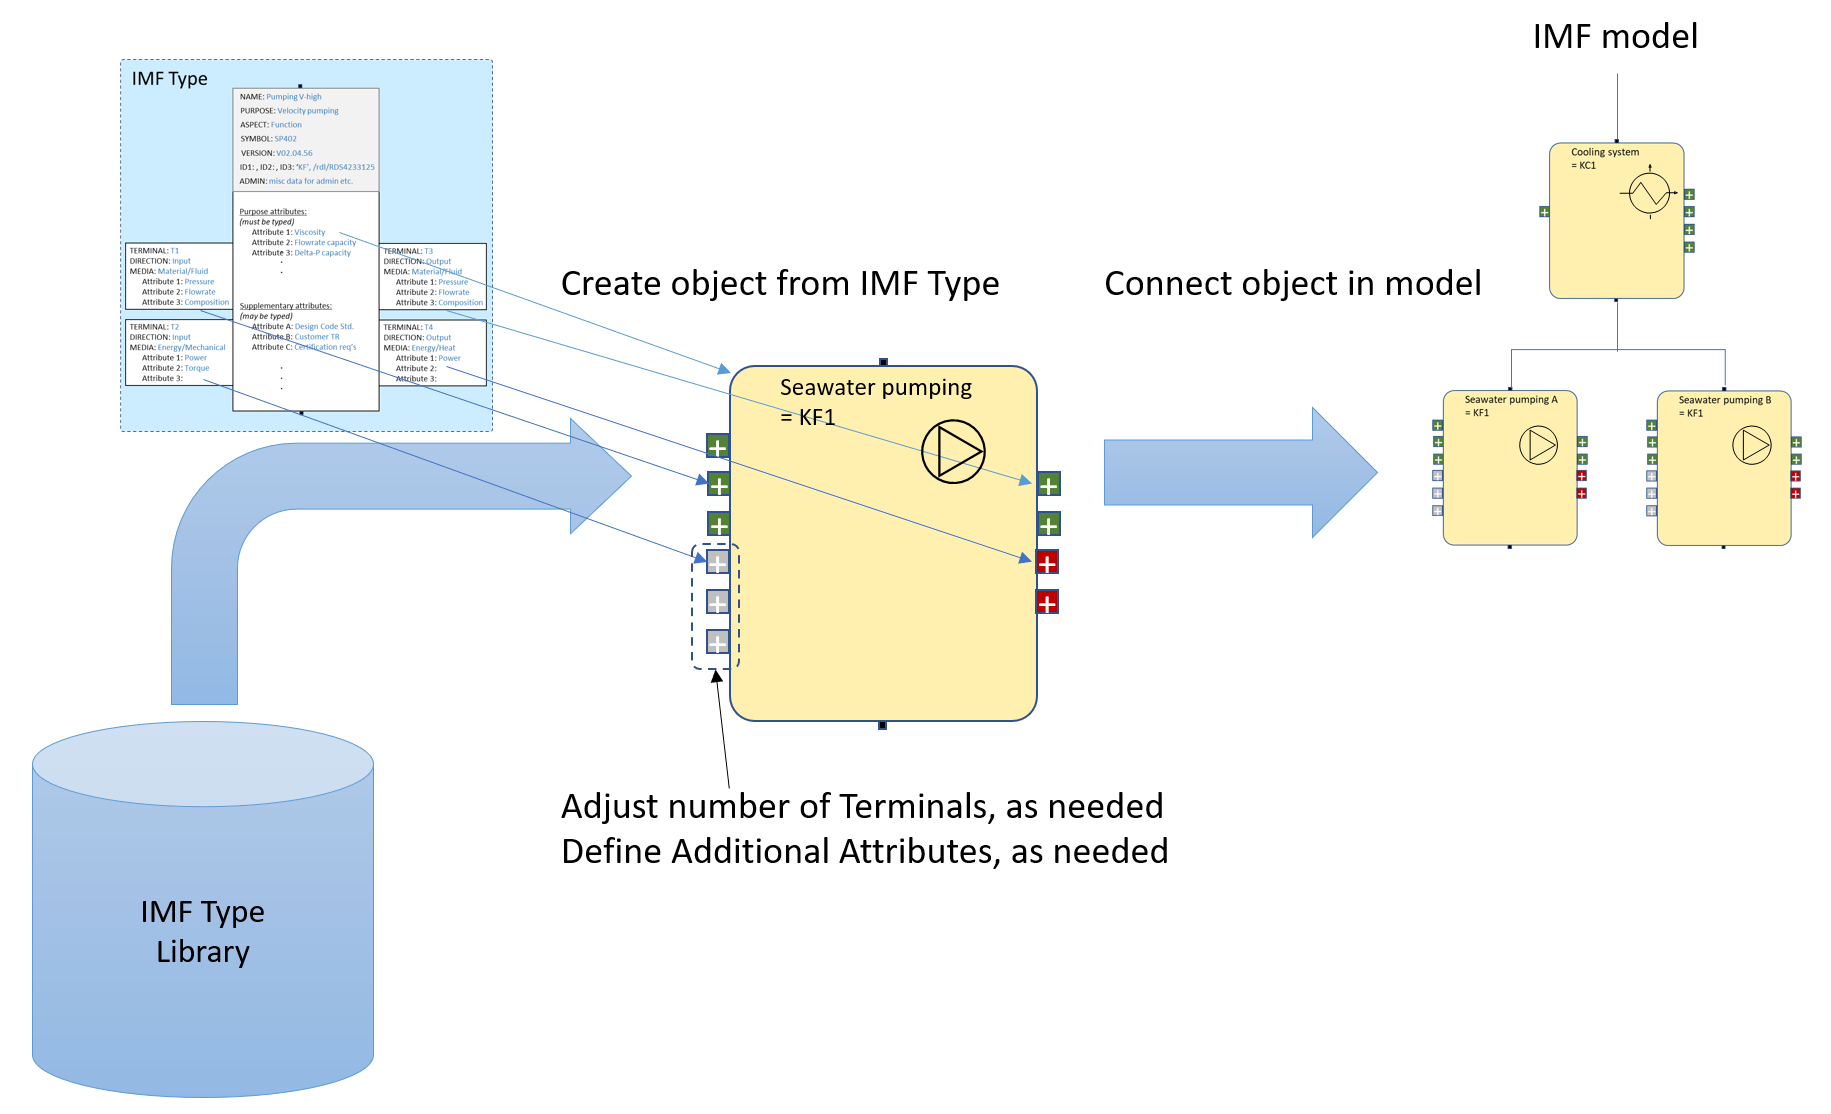
\includegraphics[width=1\textwidth]{img/IMFmanual-img0xx.png}
  \caption{Using an IMF type from a library.}
  \label{fig:Figure 38}
\end{figure}

\subsection{Selecting an IMF Type}
The IMF type library will hold a large volume of IMF types, and they represent different
levels of specialisation. For example, an IMF type Liquid Pumping represents pumping at a generic level, whereas an
IMF type Centrifugal High dp Liquid Pumping represents a much more specialised pumping. When selecting the
appropriate IMF type, it is therefore not sufficient to only select the desired purpose (in the this example: Pumping), but also the
desired level of specialisation must be chosen.

When selecting the IMF type, also its aspect must be chosen (Function, Product, Location, or Installed).

\subsection{What if the Needed IMF Type does not Exist?}
If a close enough match cannot be found between what is needed and what is available in
the IMF type library, then a new IMF type must be created. The IMF type library is a common industry resource, which
means that creating new IMF types demands access to applicable tools, as well as having the mandate; see \autoref{ch:How to Specify IMF Types}.
Other IMF type libraries than the common industry library is likely to be developed, sometimes with limited sharing.
They may be needed due to specialisation or intellectual property protection or other reasons. IMF is designed to
support such a variety of IMF type libraries.

\subsection{How to Place the Aspect Element into the Model}
When an aspect element has been created it can be placed into the model by
means of connecting it to other aspect elements. There are three main kinds of such placements/connections:

\begin{itemize}
  \item Into the hierarchy of existing aspect elements, effectively creating hierarchical relations.
  \item Into the topology of existing aspect elements, effectively creating topology relations.
  \item Into the relation between aspect elements of different aspects, effectively creating inter-aspect relations.
  \end{itemize}
  The order in which the connections are made depend on the chosen modelling approach, but ultimately all must
be made to complete a model.

\subsection{Set Attribute Values of Aspect Elements}
When a new aspect element is created from an IMF type it will have one or several
attributes of a given quality. This is provided as part of the IMF type definition. Examples of qualities are
Pressure, Temperature, Speed etc. It is possible during the modelling to increment as needed the number of
(amount) attributes of the same type, as well as specify further specialisation of attribute values, such as quantity
datum, e.g., Pressure \emph{Design, Maximum}, and sub-quality, e.g., Pressure Design Maximum,
\emph{Cavity}. It is also possible to add entirely new attributes to the aspect element, when that is needed to hold information that is not part of the basic IMF type definition. Usually this is supplementary information which is not strictly required, but is convenient to include.

\begin{figure}[htb]
  \centering
  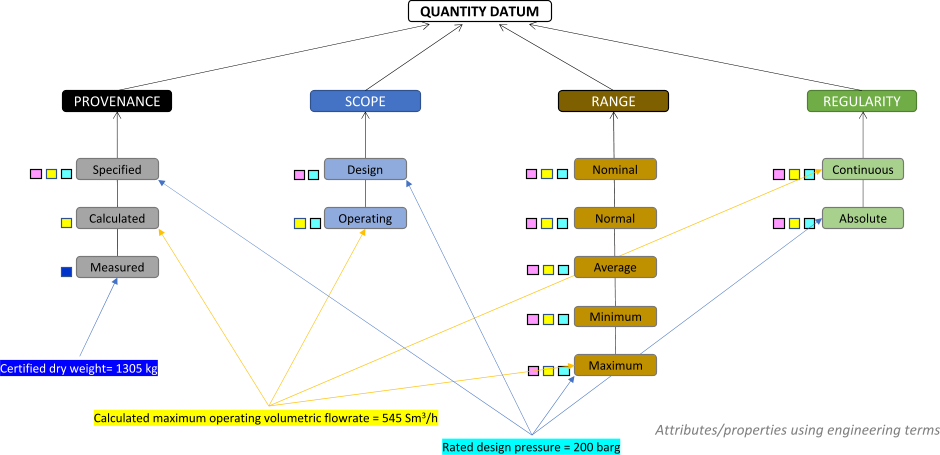
\includegraphics[width=1\textwidth]{img/IMFmanual-img058.png}
  \caption{Typing of attribute values to provide context.}
  \label{fig:Figure 39}
\end{figure}

Assigning attribute values to quantity datum classes can be done as shown in \autoref{fig:Figure 39}. Some examples are:

\begin{itemize}
  \item Pressure: Specified/Design/Maximum/Absolute
  \item Volumetric flowrate: Calculated/Operating/Maximum/Continuous
\end{itemize}
Conventional engineering terms may differ from this classification scheme, but the meaning is the same. As an example,
Rated Design Pressure corresponds to Pressure: Specified/Design/Maximum/Absolute.

Once the number of attributes has been entered and their value datum types are selected, they are ready to be given
values and units of measure can be selected. As an example, the attribute Pressure: Specified/Design/Maximum/Absolute may be
given a value of 200 barg.

Usually only a few attributes are needed to be given an actual value, to provide a sufficiently detailed description.
This must be judged in each individual case, and there are no firm rules. As an example, when defining a pumping
function, it may be essential to enter a value for the volumetric flowrate and differential pressure, as this
characterises the pumping, but it may be less important to enter a value for rotational speed as this is not about
what the pumping results in.

The above quantity datum is based on the concept of quality and quantity datum, and the types of quantity datums from
ISO~15926-14.

\subsection{Where Attribute Values Reside}

The actual attribute values may reside in the model data itself, or they may reside in
other engineering registers or applications and be available as linked data, or they may reside in external systems
and not be available as data, but only be pointed to. Where the attribute values reside therefore depends on the
actual implementation of the modelling tools and applications. Some examples of how attributes could reside in
different places:

\begin{itemize}
  \item Model data:

        \begin{itemize}
          \item Activity = Pumping
          \item Volumetric flowrate: Calculated/Operating/Maximum/Continuous = 500 m\textsuperscript{3}/h
        \end{itemize}
  \item Linked data:

        \begin{itemize}
          \item Speed = 3000 rpm [/engineering\_register/separation\_system/pump1/speed]
          \item Temperature: Calculated/Operating/Maximum/Continuous = \\ 120 {\r{}}C
                [/engineering\_register/separation\_system/separator1/temp]
        \end{itemize}
  \item Pointed-to:

        \begin{itemize}
          \item Technical Requirement Specification 0023423-55B
        \end{itemize}
\end{itemize}
This means that in some implementations \emph{all} attributes reside in the model data (could be a modelling tool
for conceptual design), whereas in some other implementations \emph{few or none of the} attributes reside in the
model data but are in external engineering registers. Most likely the most optimal solutions lie somewhere in between
the two extremes.

\subsection{Allocate Terminals}
When a new block is created it will have one or several terminals.
This is typically provided as part of the IMF type definition. A terminal can have a specified flow direction, e.g., Input or Output, and is defined by which type of media it pertains to, such as Energy/Electrical or Material/Fluid. It
is part of the modelling work process to increment as needed the number of terminals of the same type. For example,
increment to two input terminals with the media Energy/Electric.

\subsection{Setting Attribute Values on the Terminals}
Examples of qualities are Force, Voltage, Power, etc. It is part of the modelling 
process to increment as needed the number of attributes of the same quality for a terminal as needed, e.g., increment
to two Voltage attributes. Furthermore, the attribute values can be further typed by assigning them to quantity datum
classes. Examples are:

\begin{itemize}
  \item Voltage: Design/Maximum/Absolute
  \item Voltage: Operating/Normal/Continuous
\end{itemize}
Once the number of attributes has been entered and their datum types are selected, they are ready to be given values
and units of measure can be selected. As an example, the Voltage: Design/Maximum/Absolute may be given a value of 6.6
kV.

\subsection{Connecting Terminal to Terminal between
  Blocks}
Blocks will have terminals, and they are the means for modelling how streams flow.
The output terminal of one block needs ultimately to be connected to the input terminal of another block
 in order to model a stream. At the high level of the model the connection between output terminal and input terminal may simply
be viewed as a transport connection, whereas at lower levels more details could emerge, revealing that this transport
connection comprises one or several pipes, shafts, or cables, possibly with some devices, each having specific
characteristics.

\subsection{Iterate on Creating and Editing Aspect Elements}
As more and more blocks with terminals are created and connected into the IMF model it becomes
richer and richer on facility asset information. As the design progresses, it is part of a natural workflow that
aspect elements need to be edited and possibly also reconnected elsewhere in the IMF model. 
This allows for modelling to begin even when very little information is known, and then repeatedly
review and enrich the IMF model until the desired level of accuracy is reached.

\subsection{Understanding and Managing the Consequences
  of Changes}
The high level of flexibility of modelling also means that changes can be made frequently,
and this carries the risk of causing inadvertent changes. It is therefore important to understand what the potential
(possibly far-reaching) effects of a change could be. A change to one aspect element could mean that other aspect elements to which
it is connected are also affected by the change, e.g., changing something in a system is likely to affect the system
it is part of. To alleviate this, the tool used for modelling may have mechanisms that warn about such unwanted consequences.

\subsection{Conditions for Shifting the Modelling Aspect}
It is challenging to understand when to model in the Function Aspect and when to model
in the Product Aspect. In many cases there is no sharp line between them. This issue is also recognised from
document-based design processes, where the art of writing truly \emph{functional} requirements is difficult. Very
often there is a need to include some solution specifications. By principle, solution specifications shall be
modelled in the Product Aspect, but IMF modelling allows for flexibility in this regard. It does not force all
requirements to be in the Function Aspect, nor does it force all specifications to be in the Product Aspect. A
pragmatic approach should be taken, aiming at an IMF model which is fit-for-purpose.

The Location Aspect is more distinct and is entirely different from the other aspects. Because this aspect will hold
area requirements to component, equipment, or assemblies located there, there may be situations when these are
modelled in the Product Aspect and the specification reveal that they cannot meet the requirements set by their
intended location. In such cases it may be needed to shift to the Location Aspect and revise the location
requirements, alternatively to change the location. 
The Installed Aspect is solely used for documenting real world
physical objects, and how they fulfil the specifications given in the Product Aspect.

\section{Connecting Relations Between Aspects}
When working with multiple aspects it may be necessary to specify how a system is
modelled in the different aspects. This is done using inter-aspect relations, as shown in \autoref{fig:Figure 40}.

\begin{figure}[htb]
  \centering
  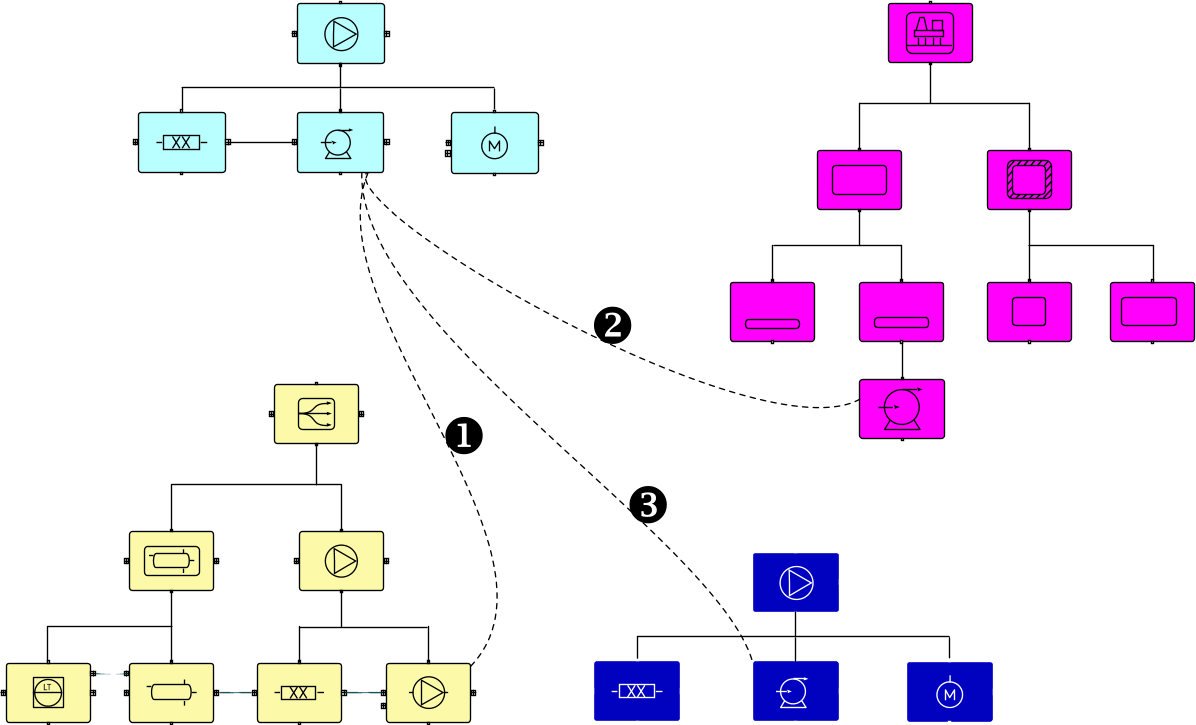
\includegraphics[width=.95\textwidth]{img/IMFmanual-img059.png}
  \caption{Inter-aspect relations.}
  \label{fig:Figure 40}
\end{figure}

The relations can be set in any order, but usually the sequence will be as per the numbering of the figure.

\begin{enumerate}
  \item The logical first step is the relation which specifies that activity requirements modelled in the Function Aspect are
        fulfilled by solution specifications modelled in the Product Aspect. In this example the requirements for the pumping
        activity are fulfilled by the specifications of the pump.
  \item The logical second step is the relation which specifies two things:

        \begin{enumerate}
          \item That the solution specification modelled in the Product Aspect occupies a specific space and has a particular
                relative position in a particular location; this is modelled in the Location Aspect. In this example the specified
                pump has a defined size and is relatively positioned in a defined location.
          \item That the solution specification modelled in the Product Aspect fulfils the location-based requirements modelled
                in the Location Aspect. In this example the specified area where the pump is located is specified as exposed to
                weather and is met by the pump being specified as weatherproof.
        \end{enumerate}

Note that for the Location Aspect requirements are given by the parent block, e.g., when a pump is
located in a process area it is the requirements of that process area that apply to the pump.

  \item The relation between the Product Aspect and the Installed Aspect serves to document that an actual component,
        equipment, or assembly fulfils the solution specified. Note that there may be several fulfilling the same
        specification, as is the case for spares in storage.
\end{enumerate}
Not all aspect elements will have relations to other aspects. A function block which is modelling a large
system will almost never have a relation to a single solution specified as a product block. And an area or room or other such location
modelled as a location block will almost never have a relation to a single solution specified as a product block.

\subsection{Connect Function--Product Relation}
When the requirements to a system of activities have been broken down to such a level of
detail through modelling that it is feasible to fulfil the requirements in a solution specification, then a relation
between requirement and solution can be established. This is done by connecting the relation between the function
block representing the requirements, and the product block representing the solution specification.

\subsection{Connect Product--Location Relation}
When the arrangement of the intended locations (rooms, areas, etc.) have been modelled to
such a level of detail that a location is available for a specified solution, then a relation between location and
solution can be established. This is done by connecting the relation between the product block representing
the solution, and the location block representing the spatial properties of the solution, \emph{and} by
connecting the location block into the location block hierarchy, i.e., stating which location it is part of.

\subsection{Connect Product--Installed Relation}
When a component, equipment, or assembly is manufactured, delivered, or installed, the
documentation of it can be linked to its solution specification, by means of connecting a relation between the
installed block representing the actual component, equipment, or assembly, and the product block
representing the solution specification.

\subsection{Connect Relations to other Aspects}
A facility asset model can be further augmented by introducing new aspects, such as an
\emph{Engineering Numbering Aspect (TAG Aspect)} which can enable relations between requirements, solutions, locations, and
their nameplate TAG numbers. Likewise, a \emph{Maintenance Aspect} can enable relations between component, equipment, or
assembly and their maintenance task. New aspects can be created based on simple rules and components (planned in a
later version).

Connecting relations to these possible future blocks will follow the same principle but this is yet to be defined.

\section{IMF Model Integration}
IMF allows for modelling smaller IMF models that later are integrated into larger models,
as conceptually shown in \autoref{fig:Figure 41}. More advanced mechanisms for supporting this are planned described for a later version of
IMF. The integration can be between models in different aspects (1) or between different multi-aspect models (2).

\begin{figure}[htb]
  \centering
  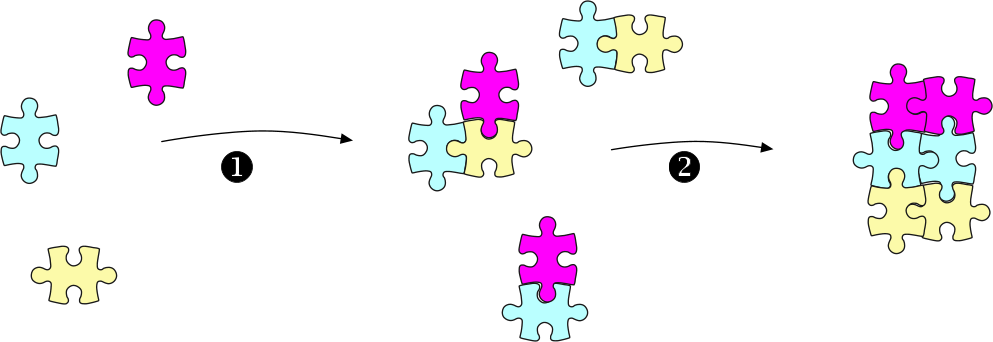
\includegraphics[width=.96\textwidth]{img/IMFmanual-img060.png}
  \caption{The concept of model integration.}
  \label{fig:Figure 41}
\end{figure}

This supports a work process where the design work is split into different resources for later to be integrated into a
whole. The integration between aspects is achieved through connecting relations between aspects, as described in
previous sections, whereas integrating different multi-aspect models requires managing somewhat complex interfaces
between the models. The integration of several models in the same aspect is simply achieved by placing them into a
common hierarchy.

\subsection{Managing Integration of two IMF Models}
Integrating one IMF model with another IMF model requires managing the interfaces between
the two models, as highlighted with focus rings in the figures.

\begin{figure}[htb]\centering
  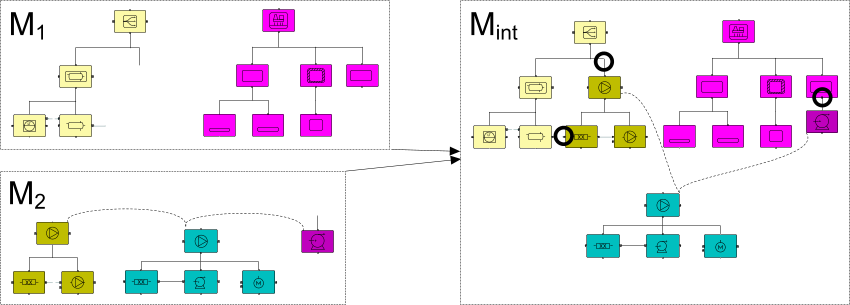
\includegraphics[width=1\textwidth]{img/IMFmanual-img061.png}
  \caption{Model integration.}
  \label{fig:Figure 42}
\end{figure}

When IMF model M\textsubscript{1} is integrated with the higher-level IMF model M\textsubscript{2} what results is
the integrated result of the two, M\textsubscript{int}. To do this successfully all the connecting points or
interfaces must be carefully managed through appropriate modelling.

\section{IMF Model Examples}
\subsection{A Process Performance
  Requirement Model}
This example is a simple three-phase hydrocarbon separation system where the water level
is controlled by pumping. The interest of this modelling is to describe the system and its performance requirements.
To do this, the entire system and the individual sub-systems needed as part of it are modelled, namely the separation
activity, the pumping activity, and the controlling activity. No decisions regarding a solution specification are
made, and therefore the entire model is placed in the Function Aspect. The model is illustrated in \autoref{fig:Figure 43}.

\begin{figure}[htb]
  \centering
  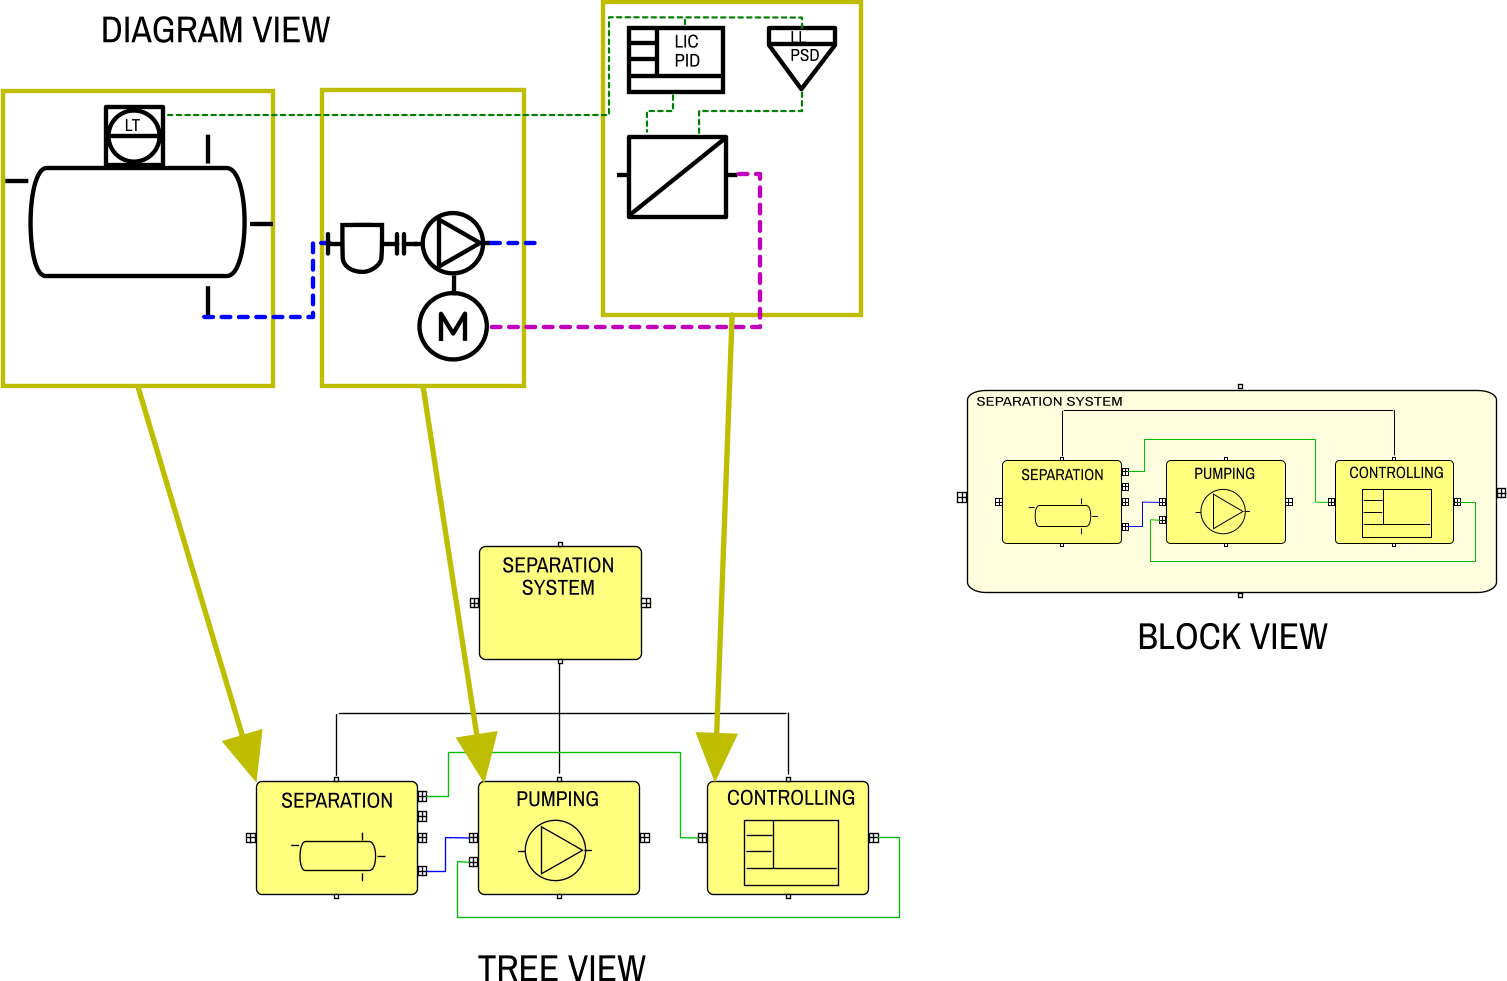
\includegraphics[width=1\textwidth]{img/IMFmanual-img062.png}
  \caption{Separation system modelled in Function Aspect.}
  \label{fig:Figure 43}
\end{figure}

The function aspect hierarchy defines the system breakdown structure, and the streams define how the systems are
connected together. Each of the function blocks define the requirements to what they represent, e.g., the
Pumping function block defines the requirements to the pumping activity, such as required flowrate and
differential pressure. To set these requirements by modelling is done by assigning values to the attributes of the
function block, e.g., by setting the attribute Differential Pressure to 20 bar.

Requirements are defined at different levels of detail, as shown in this example, where the entire separation system
is represented at a high level by one Separation System function block. At this level the stated
requirements could be limited to the required capacity to perform separation of crude oil of a specified quality.

To help interpret the figure, the same processing plant is shown in three different views: Diagram View is for
similarity with the formats known from drawings such as process flow diagrams and system control diagrams. Tree View is a view of the model which emphasises the breakdown structure, and Block View is a view of the
model which emphasises the topology (streams). If there is a need for further detailing the requirement, such as for
the pumping performance, further breakdown of the pumping system could be modelled, e.g., by breaking down Pumping
into Filtering, Pumping, and Driving, each represented by a function block.

\subsection{A Multi-Discipline Requirements-Thread Model}
This example is a process facility, and the emphasise is on how modelling is directed by
the thread of requirements, as illustrated by the red line in \autoref{fig:Figure 44}. No decisions regarding a solution
specification are made, and therefore the entire model is placed in the Function Aspect.

\begin{figure}[htb]\centering
  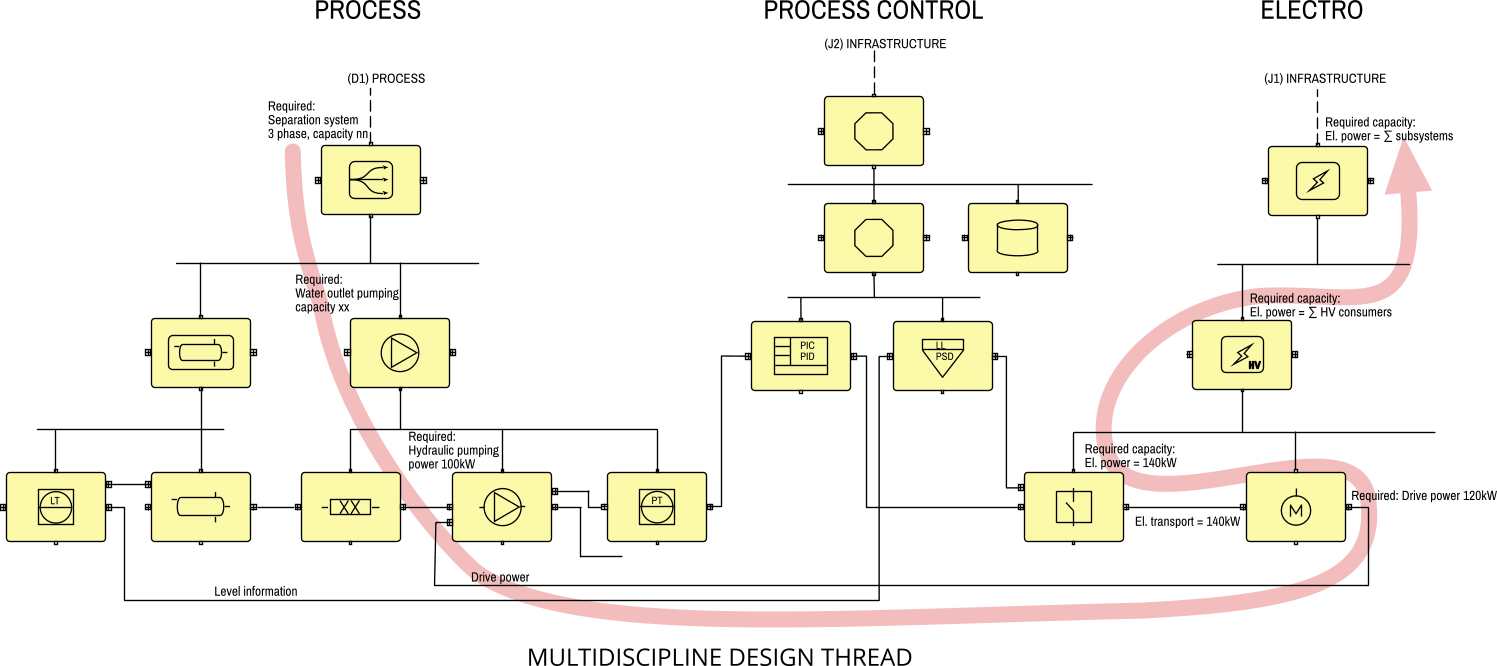
\includegraphics[width=1\textwidth]{img/IMFmanual-img063.png}
  \caption{Modelling directed by the thread of requirements.}
  \label{fig:Figure 44}
\end{figure}

This particular requirement thread ties high level process requirements to high level electro requirements. Other
requirement threads (not shown) similarly lead from process to process control. In the example the separation
requirement is broken down into Separation, and Pumping. Pumping requires mechanical energy, so it must be connected
to Driving (motor). Driving requires controlled electrical energy, so it is connected to electrical distribution
through Switch. The required electrical energy adds to the required total electrical energy capacity of the
facility. As can be seen from this exercise, the conventional division into different disciplines is irrelevant, and
instead a multi-discipline approach is invited.

\subsection{A Catalogue Equipment Specification}
This example is of a small centrifugal pump including an electrical motor. It is a
catalogue product, and the purpose of the modelling is to build a specification of this solution, which shall
potentially fulfil some customer's requirement to pumping. The example is illustrated in \autoref{fig:Figure 45}.

\begin{figure}[htb]\centering
  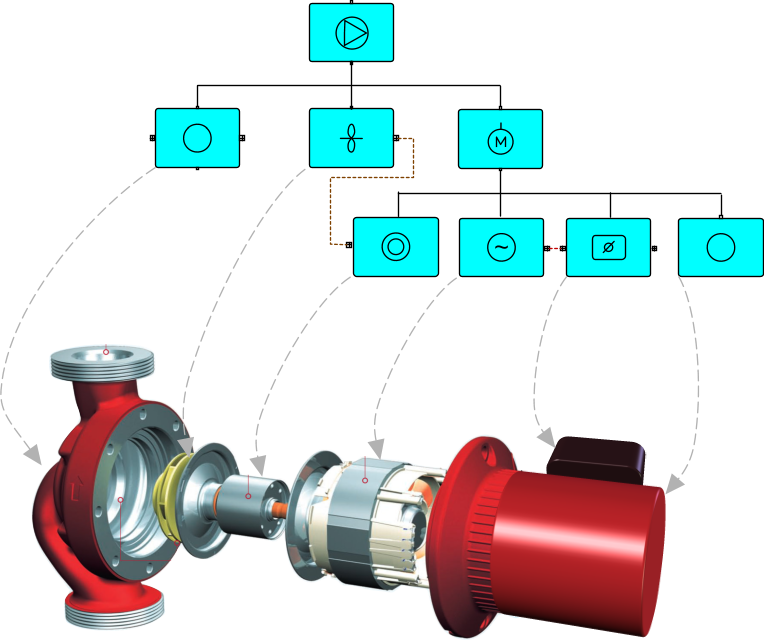
\includegraphics[width=.8\textwidth]{img/IMFmanual-img064.png}
  \caption{Pump product model.}
  \label{fig:Figure 45}
\end{figure}

For illustration the pump is shown in exploded view. It comprises, from left to right, a pump housing, an
impeller, a motor rotor, a motor stator, a motor housing, and a motor termination box.  In the model, the breakdown
specifies the assembly of these parts. Each part shown is represented by a product block, which provides a
specification of that part, including input and outputs specified as terminals. Pump Housing has an inlet
and an outlet, which is represented as input terminal and output terminal that specify attributes such as connection
type and dimension. Motor Rotor has an output of type Energy/Mechanical/Rotating which here is connected to 
Impeller Input. Not all such connections are shown (for clarity) including the mounting of the motor housing to the
pump housing, which would be modelled as input and output terminals of type Force/Mechanical.

Likely one or several of the parts are also used for other catalogue pumps, in which case they need only be modelled
once, and be reused across a range of pumps.

The level of detail of specification is dependent on the use case, and IMF allows any level of modelling to be done,
both as regards breakdown into smaller parts, as well as how rich the set of attributes for each part is.

\subsection{A Facility Asset Architecture Model}
This example is of the area architecture of an oil \& gas production platform. The
drawings in \autoref{fig:Figure 46}  show a side view and several elevation views of the facility. Information about the location
of components, equipment, and assemblies are shown as TAG numbers on the drawing, but without exact positions.
Information about the requirements given by a location, such as the open weather conditions on the weather deck is
not shown at all in such a document format. The purpose of modelling this architecture in the Location Aspect is to
specify all such information in the context of the location.

\begin{figure}[htb]
  \centering
  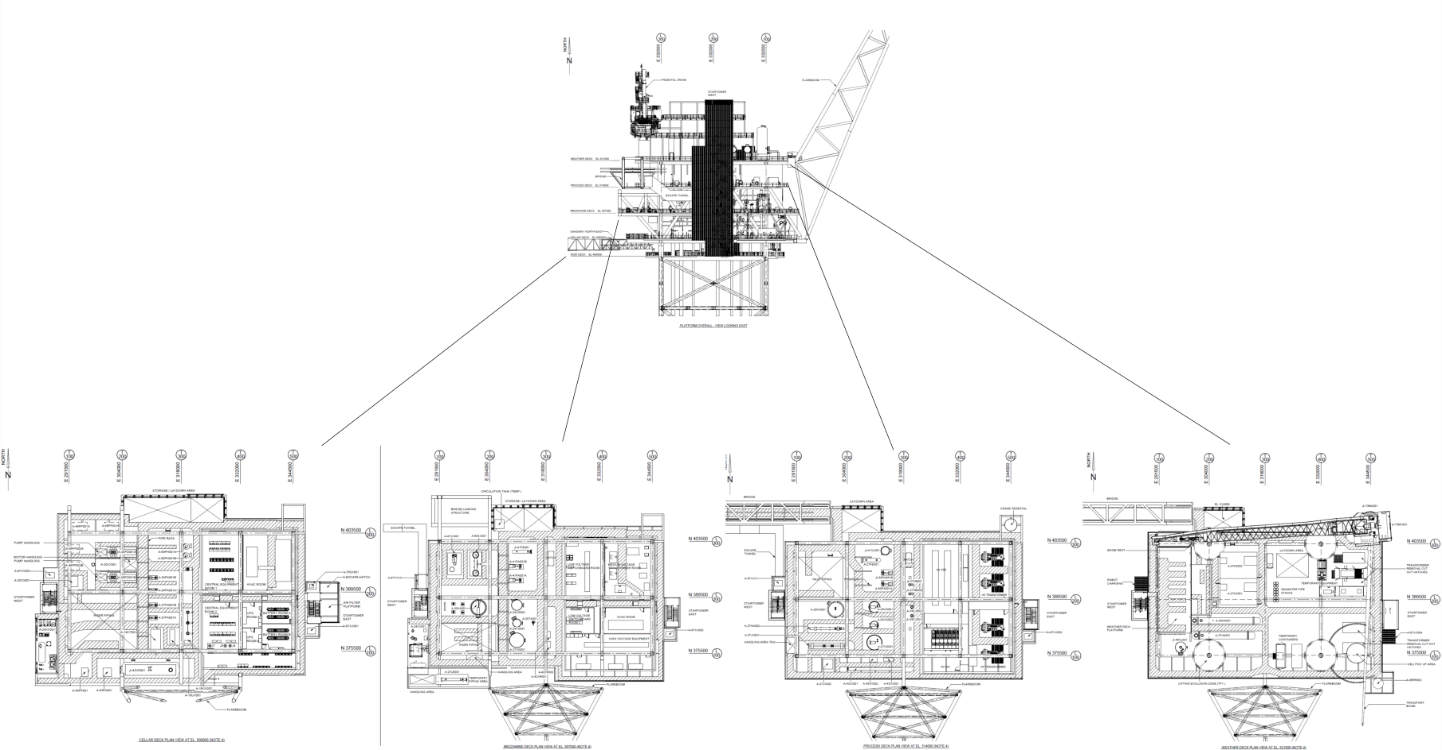
\includegraphics[width=1\textwidth]{img/IMFmanual-img065.png}
  \caption{Plot plans for a platform.}
  \label{fig:Figure 46}
\end{figure}

\begin{figure}[htb]\centering
  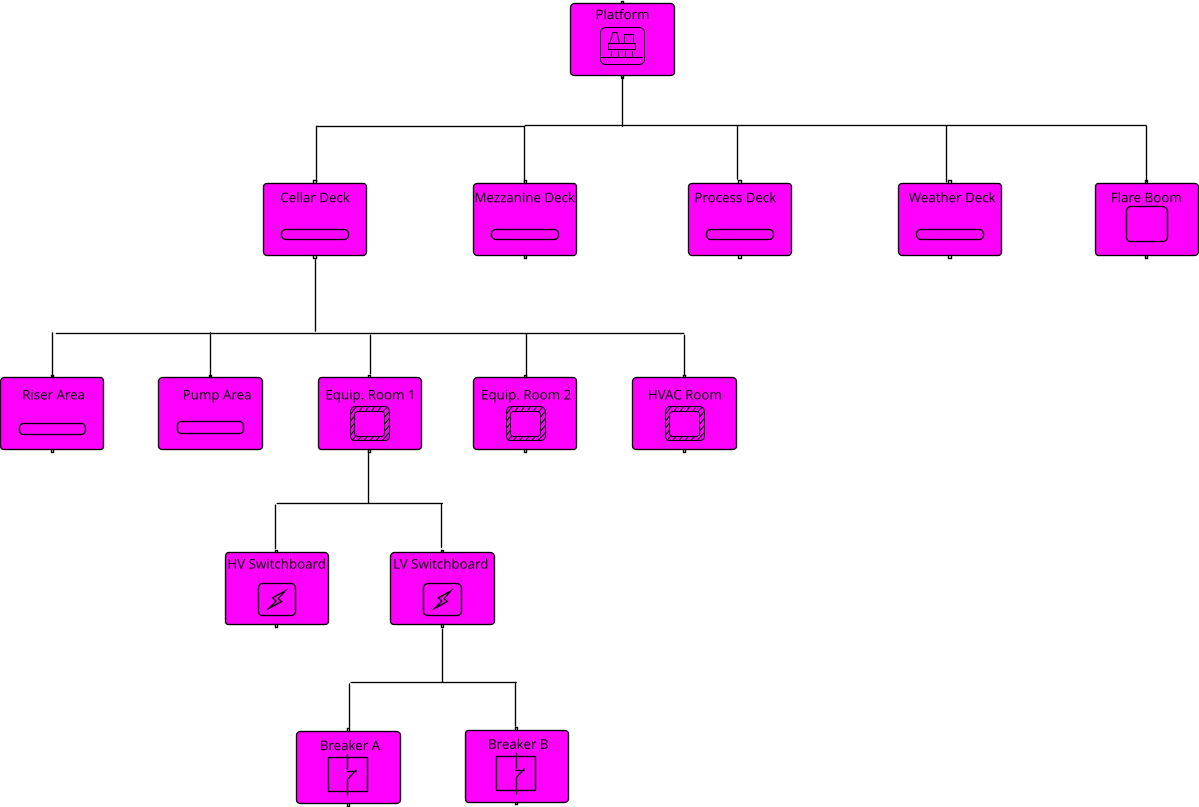
\includegraphics[width=1\textwidth]{img/IMFmanual-img066.png}
  \caption{Model in Location Aspect.}
  \label{fig:Figure 47}
\end{figure}


To model a facility asset architecture the best approach is to begin at the top, in this case the platform, and then
break down into decks, modules, areas, rooms---until the level of detail is reached when all the components,
equipment, and assemblies that is or will be modelled in the Product aspect can be placed in locations, i.e.,
modelled in the Location Aspect.

\autoref{fig:Figure 47} shows how the platform shown on the plot plan drawings can be modelled in the Location Aspect. For clarity only
one location has been broken down to a level of detail ready for locating components, equipment, and assemblies, in
this case, electrical equipment. In this example Equipment Room 1 is likely to be stated as dry, ventilated, and
cooled area. This means that there is no requirement to the switchboards located there to be waterproof. Note that if
the LV Switchboard were to be relocated to the weather deck it would be subject to the conditions and requirements in
that area and would likely be required to be waterproof.

\section{Employing Re-usable Design Patterns}
\label{sec: Employing Re-usable Design Patterns}
Usually, the design of industrial facilities is done by configuring a selection of
preexisting solutions, or \emph{design patterns}. Whenever it is an option to re-use preexisting designs, there
is a need to do this as efficiently as possible. To accommodate this, \emph{IMF complex types} offer a means to encode such
typical design patterns in the form of a template---at the level of granularity and detail desired.

\subsection{Design Patterns in Engineering}
A design pattern in engineering refers to a typical design which is likely to be re-used.
It may have emerged as a de facto typical resulting from repeated use within a particular domain, or it may be more
formalised such as being specified in a standard. It may be typical across the industry, or it may be a proprietary
design re-used within a company. It may be complex and large, such as a Gas Compression Package, or it may be very
limited in scope, such as an Electrically Driven Pump. In most cases it is valuable to include more than one aspect
to fully describe a design pattern. Also, it may be valuable to specify the breakdown structure within each aspect.
As such a IMF complex type may appear similar to a small facility asset Model. However, a design pattern is not a \emph{copy} of a
previous design, instead it is a description of that which is repeated across several previous and similar designs,
thus emerging as a typical. To achieve such a description a breakdown structure may need to be included, but the
individual elements in the breakdown structure may only require the attribute Purpose to be specified.
Optionally type and attribute information can be included for the elements in the breakdown structure, or it can be deferred to a later stage, depending on the work
process.

\subsection{Design Patterns represented as IMF Complex Types}
IMF complex types differ from (basic) IMF types in that they allow more than one aspect to be
specified, and they allow specifying a breakdown structure for each of the aspects included.  As an example, the IMF
complex type for the Electrically Driven Pump as a design pattern could specify both the Function and Product
Aspects, with their main purpose, attributes and terminals, and furthermore specify the breakdown into Electric Motor,
Shaft\& Coupling, and Pump Unit---with their Purpose attributes set to Drive, Transport, and Pump, respectively. This would reflect
the general design pattern that is used every time an Electrically Driven Pump is incorporated into an IMF model
but would not include specifics related to the particular application.

\subsection{Modelling Using IMF Complex Types}
When modelling a facility asset where a part of the model can be created by re-using an
established design pattern, this is done by creating an instance of the design pattern from an IMF
complex type. These are fetched from a library, or more precisely they are created from definitions called IMF
complex types that reside in the IMF type library. When such a design pattern is created it defines a minimum of
terminals, attributes, breakdown structures, and possibly also some topology, but the full details related to the
particular application are not defined. These details may be completed at this stage or be deferred to later stages
in the design process. The design pattern must then be tied into the model breakdown hierarchy where appropriate, and
be connected between terminals, so that it becomes an integrated part of the overall model.

\subsection{Deferred Setting of Attributes}
To defer or postpone the setting of attributes can be a powerful feature when modelling.
It allows deciding breakdown structure before details of the individual elements in the breakdown structure are
known. The minimum information can be limited to stating the Purpose of each block with terminals and how they are related
in a breakdown hierarchy. This can be progressively enriched at later stages by deciding which IMF type each aspect
element shall be, followed by deciding on terminals, attributes, and topology information.  The breakdown structure
can also be further developed into a higher level of granularity as design progresses.

\end{document}
